\documentclass[varwidth=true, border=2pt]{standalone}

\usepackage{pgfplots}
\usepackage{tikz}

\usetikzlibrary{calc,patterns,angles,quotes}

\begin{document}
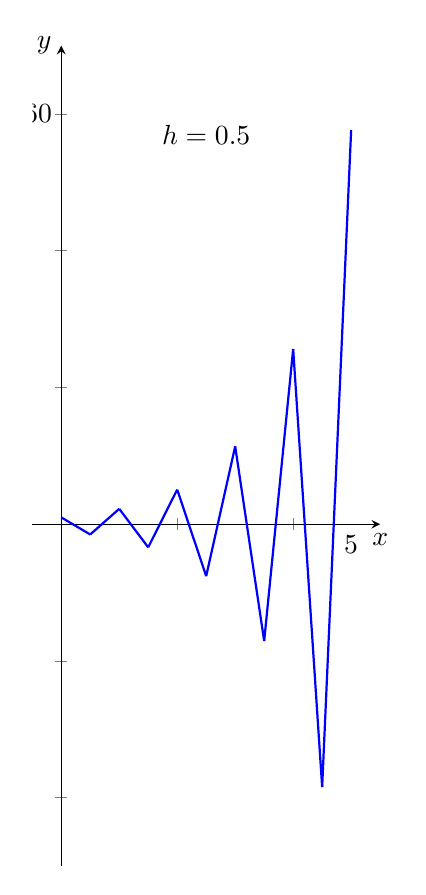
\begin{tikzpicture}
    \begin{axis}[
        legend pos=south east,
        axis x line=middle,
        axis y line=middle,
	every axis x label/.style={at={(current axis.right of origin)},anchor=north},
	every axis y label/.style={at={(current axis.above origin)},anchor=east},
	xticklabels=\empty,
	yticklabels=\empty
        grid = none ,
        width=6cm,
        height=12cm,
        grid style={dashed, gray!1},
        xmin=0,     % start the diagram at this x-coordinate
        xmax=5,    % end   the diagram at this x-coordinate
        ymin=-40,     % start the diagram at this y-coordinate
        ymax=60,   % end   the diagram at this y-coordinate
        xlabel=$x$,
        ylabel=$y$,
        enlargelimits=true,
   %     xtick={0.1, 0.2, 0.3, 0.4, 0.5, 0.6, 0.7, 0.8, 0.9, 1},
        tension=0.08]


         %\addplot[domain=-0.2:2.1625, gray,samples=250, thick] {exp(-5*x)};
         
         %  Step Size h = 1
         \node (X0) at (axis cs: 0,1) {};

         \node (B1) at (axis cs: 0.5,-1.5) {};
         \node (B2) at (axis cs: 1,2.25) {};
         \node (B3) at (axis cs: 1.5,-3.375) {};
         \node (B4) at (axis cs:2,5.0625) {};
         \node (B5) at (axis cs:2.5,-7.59375) {};
         \node (B6) at (axis cs:3,11.390625) {};
         \node (B7) at (axis cs:3.5,-17.085938) {};
         \node (B8) at (axis cs:4,25.6289063) {};
         \node (B9) at (axis cs:4.5,-38.443359) {};
         \node (B10) at (axis cs:5,57.6650391) {};
         \draw [thick,blue] (X0.center) to (B1.center);                    
         \draw [thick,blue] (B1.center) to (B2.center);
         \draw [thick,blue] (B2.center) to (B3.center);         
         \draw [thick,blue] (B3.center) to (B4.center);
         \draw [thick,blue] (B4.center) to (B5.center);
         \draw [thick,blue] (B5.center) to (B6.center);         
         \draw [thick,blue] (B6.center) to (B7.center);
         \draw [thick,blue] (B7.center) to (B8.center);
         \draw [thick,blue] (B8.center) to (B9.center);         
         \draw [thick,blue] (B9.center) to (B10.center);
         
     %    \node (y0) at (axis cs: -0.1, 1000000){$10^6$}
         \node (x1) at (axis cs: 5, -3){5};
         \node (y1) at (axis cs: -0.4, 60){60};
                  \node (H) at (axis cs: 2.5, 57){$ h = 0.5 $};
         


    \end{axis}
\end{tikzpicture}
\end{document}